\documentclass[	11pt, ]{fphw}

\usepackage[utf8]{inputenc} 
\usepackage[T1]{fontenc}
\usepackage{mathpazo}\usepackage{graphicx} 
\usepackage{booktabs} 
\usepackage{listings} 
\usepackage{amsmath}
\usepackage{eso-pic}
\usepackage{array}
\usepackage{float}
\usepackage{graphicx}
\usepackage{bbm}
\usepackage{transparent}
\usepackage{indentfirst}
\usepackage{amsthm}
\usepackage{amsmath,amssymb}
\usepackage{subfigure}
\usepackage{tabu}
\usepackage{enumitem}
\usepackage{caption,tabularx,booktabs}
\usepackage{enumerate} 
\usepackage[english]{varioref}

\renewcommand{\thesection}{\Roman{section}}
\usepackage{titlesec}
\titleformat{\section}
{\normalfont\Large\bfseries}{Exercise~\thesection}{1em}{}
\makeatletter
\renewcommand{\@seccntformat}[1]{%
  \csname the#1\endcsname
  \csname suffix@#1\endcsname % this does nothing unless \suffix@... is defined
  \quad
}
% the subsection number is just a letter
\renewcommand{\thesubsection}{\alph{subsection}}
% but references will also have “section.subsection.” in front of the letter
\renewcommand{\p@subsection}{\thesubsection.}
% define \suffix@subsection
\newcommand{\suffix@subsection}{)}
\makeatother

\title{Assignment \#3} %
\author{Anita Mezzetti} 
\institute{École polytechnique fédérale de Lausanne} 
\class{Global Business Environment} 
\professor{Luisa Lambertini} 

%--------------------------------------------------------------------
\begin{document}
\maketitle 
\section{}
\subsection{}
The equilibrium spot exchange rate (E=current exchange rate) is the one that adjust to make sure that this equilibrium is respected. Remember that $E=E_{domestic/foreign}$, $R=R_{domestic}$ and $R^{*}=R_{foreign}$.
\[ R = R^{*} + \frac{E^{e}-E}{E}\]
We want 
\begin{equation} \label{a}
E= \frac{E^{e}}{1-R^{*}+R} 
\end{equation}
Substituting the datas:
\begin{equation}  
E = \frac{ 1.2 }{ 1- (0.04/4) + (0.03/4) }  = 1.2030
\end{equation}

The rounded (to two decimal digits) result is 1.20. 

\subsection{}
The expected exchange rate in 3 months is slightly smaller than the spot one.
\[ E^{e}-E= 1.2 - 1.2030 = -0.003 \]
So, there is a super small appreciation.
\par However, the exercises says to round off the results to two decimal digits. In this case, the difference would be zero: there is neither an appreciation nor a depreciation. 


\subsection{}
Consider R=0.02. Using the formula \ref{a}, the new E is: 
\begin{equation} 
\begin{aligned}    
E & = \frac{E^{e}}{1-R^{*}+R} = \\
  & = \frac{ 1.2 }{ 1- (0.04/4) + (0.02/4) } =\\
  & = 1.2060
\end{aligned} 
\end{equation}
The rounded (to two decimal digits) result is 1.21. See the Figure \vref{1}. It shows that a decrease in the domestic rate causes a new equilibrium point. The spot exchange rate has increased (depreciation). 

\begin{figure}[h] 
\centering 
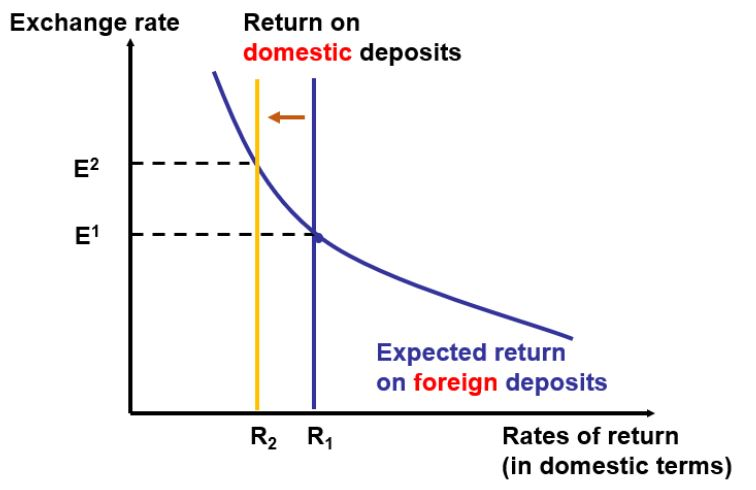
\includegraphics[scale=0.7]{figc.JPG} 
\caption{Question 1.c} 
\label{1}
\end{figure}

\subsection{}
Consider $R^{*}$=0.05 and R=0.03. Using the formula \ref{a}, the new E is:
\begin{equation} 
\begin{aligned}    
E & = \frac{E^{e}}{1-R^{*}+R} = \\
  & = \frac{ 1.2 }{ 1- (0.05/4) + (0.03/4) } =\\
  & = 1.2060
\end{aligned} 
\end{equation}
The rounded (to two decimal digits) result is 1.21. See the Figure \vref{2}.It shows that an increase in the foreign interest rate causes a shift of the expected return on foreign deposits and a new equilibrium point at a bigger exchange rate (depreciation).

\begin{figure}[h] 
\centering 
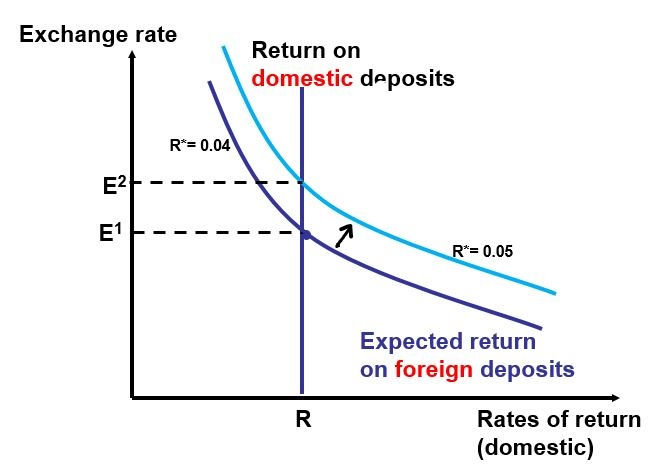
\includegraphics[scale=0.5]{figd.jpg} 
\caption{Question 1.d} 
\label{2}
\end{figure}

\subsection{}
Consider $R^{*}$=0.04, R=0.03 and $E^{e}$=1. 
Using the formula \ref{a}, the new E is: 
\begin{equation} 
\begin{aligned}    
E & = \frac{E^{e}}{1-R^{*}+R} = \\
  & = \frac{ 1 }{ 1- (0.04/4) + (0.03/4) } =\\
  & = 1.0025
\end{aligned} 
\end{equation}
The rounded (to two decimal digits) result is 1.00. See the Figure \vref{3}. It shows that a decrease in the expected exchange rate causes a shift of the expected return on foreign deposits and a new equilibrium point at a smaller spot exchange rate (appreciation). 

\begin{figure}[h] 
\centering 
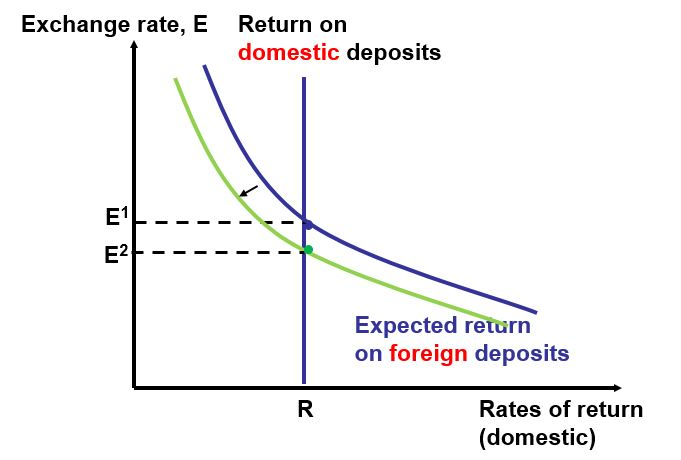
\includegraphics[scale=0.75]{fige.JPG} 
\caption{Question 1.e} 
\label{3}
\end{figure}

%---------------------------------------
\section{}
\subsection{}
\[ E^{e}_{CHF/EUR}= 0.4 * 1.1 + 0.6 * 1.016667 = 1.05 \]

\subsection{}
Using the formula \ref{a}, the spot exchange rate $E_{CHF/EUR}=E$ is: 
\begin{equation} 
\begin{aligned}    
E & = \frac{E^{e}}{1-R^{*}+R} = \\
  & = \frac{1.05}{ 1- (0.115/4) + (0.04/4) } =\\
  & = 1.070
\end{aligned} 
\end{equation}


\subsection{}
The invoice is of 1000EUR. We have to decide between three alternatives: 
\begin{enumerate}
    \item Buy the call option today: \\
    If I buy the option today I spend 0.0312CHF for 1EUR. Today I spend: 
    \[ number of EUR * 0.0312CHF = 31.2 CHF. \]
    Moreover I have to buy the EUR at the specified time settled. \\
    I consider that $E^{e}_{CHF/EUR}=1.070$. I would like to have an exchange rate as small as possible (so I need less CHF to buy the EUR). \\
    I would use my option only if $E^{e}=1.1$ (probability=0.4), using the strike price 1.04. In the other case (probability=0.6) $E^{e}=1.016667$ I would not. So,
     \[ 0.4* \frac{1000EUR*1.04CHF/EUR}{1+R/4}+0.6* \frac{1000EUR*1.016667CHF/EUR}{1+R/4}= 1015.84CHF. \]
     In the end I have a present value of  \[ 31.2 CHF+1015.84CHF= 1047.04 CHF.\]
     
    \item Buy EUR today: \\
    I need 1000EUR in 3 months. So today I buy the amount of EUR that will have a value of 1000EUR in 3 months: 
    \[ \frac{1000EUR}{1+R^{*}/4} =  \frac{1000EUR}{1+0.115/4} = 972.05 EUR\]
    I am working in CHF. Considering the spot exchange rate $E^{e}_{CHF/EUR}=1.070$, I have \[ 972.05 EUR*1.070CHF/EUR= 1040.155 CHF.\]
    
    
    \item Buy EUR in three months: \\
     I need 1000EUR in 3 months and I directly buy them. In this case we keep our CHF and we invest them. At that time 1000EUR will have a value in CHF of $1000EUR*E^{e}_{CHF/EUR}$. This amount today has a value of
     \[ \frac{1000EUR*E^{e}_{CHF/EUR}}{1+R/4}=\frac{1000EUR*1.05CHF/EUR}{1+0.04/4}= 1039.60 CHF. \]
\end{enumerate}
The cheapest alternative is the last one.


%---------------------------------------
\section{}
\subsection{}
The CIRC states that 
\[ R_{USD}^{6}=R_{EUR}^{6}+\frac{F_{USD/EUR}^{6}-E_{USD/EUR}}{E_{USD/EUR}};
\]
where $R^{6}$ is the rate of interest for six months. Then
\[\begin{aligned}
    F_{USD/EUR}^{6}&=  E_{USD/EUR}*(1+R_{USD}^{6}-R_{EUR}^{6})= \\
                    &= 1.1489* (1 + 0.02623/2 + 0.00313/2)= 1.166
\end{aligned}\]


\subsection{}
Following the formula for the forward premium, I obtain 
\[ \frac{F_{USD/EUR}^{6}-E_{USD/EUR}}{E_{USD/EUR}}=\frac{1.166-1.1489}{1.1489}= 0.015. \]
A forward premium is a situation in which the expected future price for a currency is greater than the spot price. So the market expects a depreciation of the USD relative to the EUR.








\end{document}